
\section{Analiza systemu}

Celem projektu była analiza możliwości przetwarzania równoległego w architekturze czwórki z początkowymi danymi w dolnym węźle $P1$ (jak pokazano na rysunku \ref{fig:schema}).
W ramach projektu zajmowaliśmy się dwoma modelami - sekwencyjnym oraz równoległym z jedną komunikacją na łączu.

\begin{figure}[!ht]
\centering
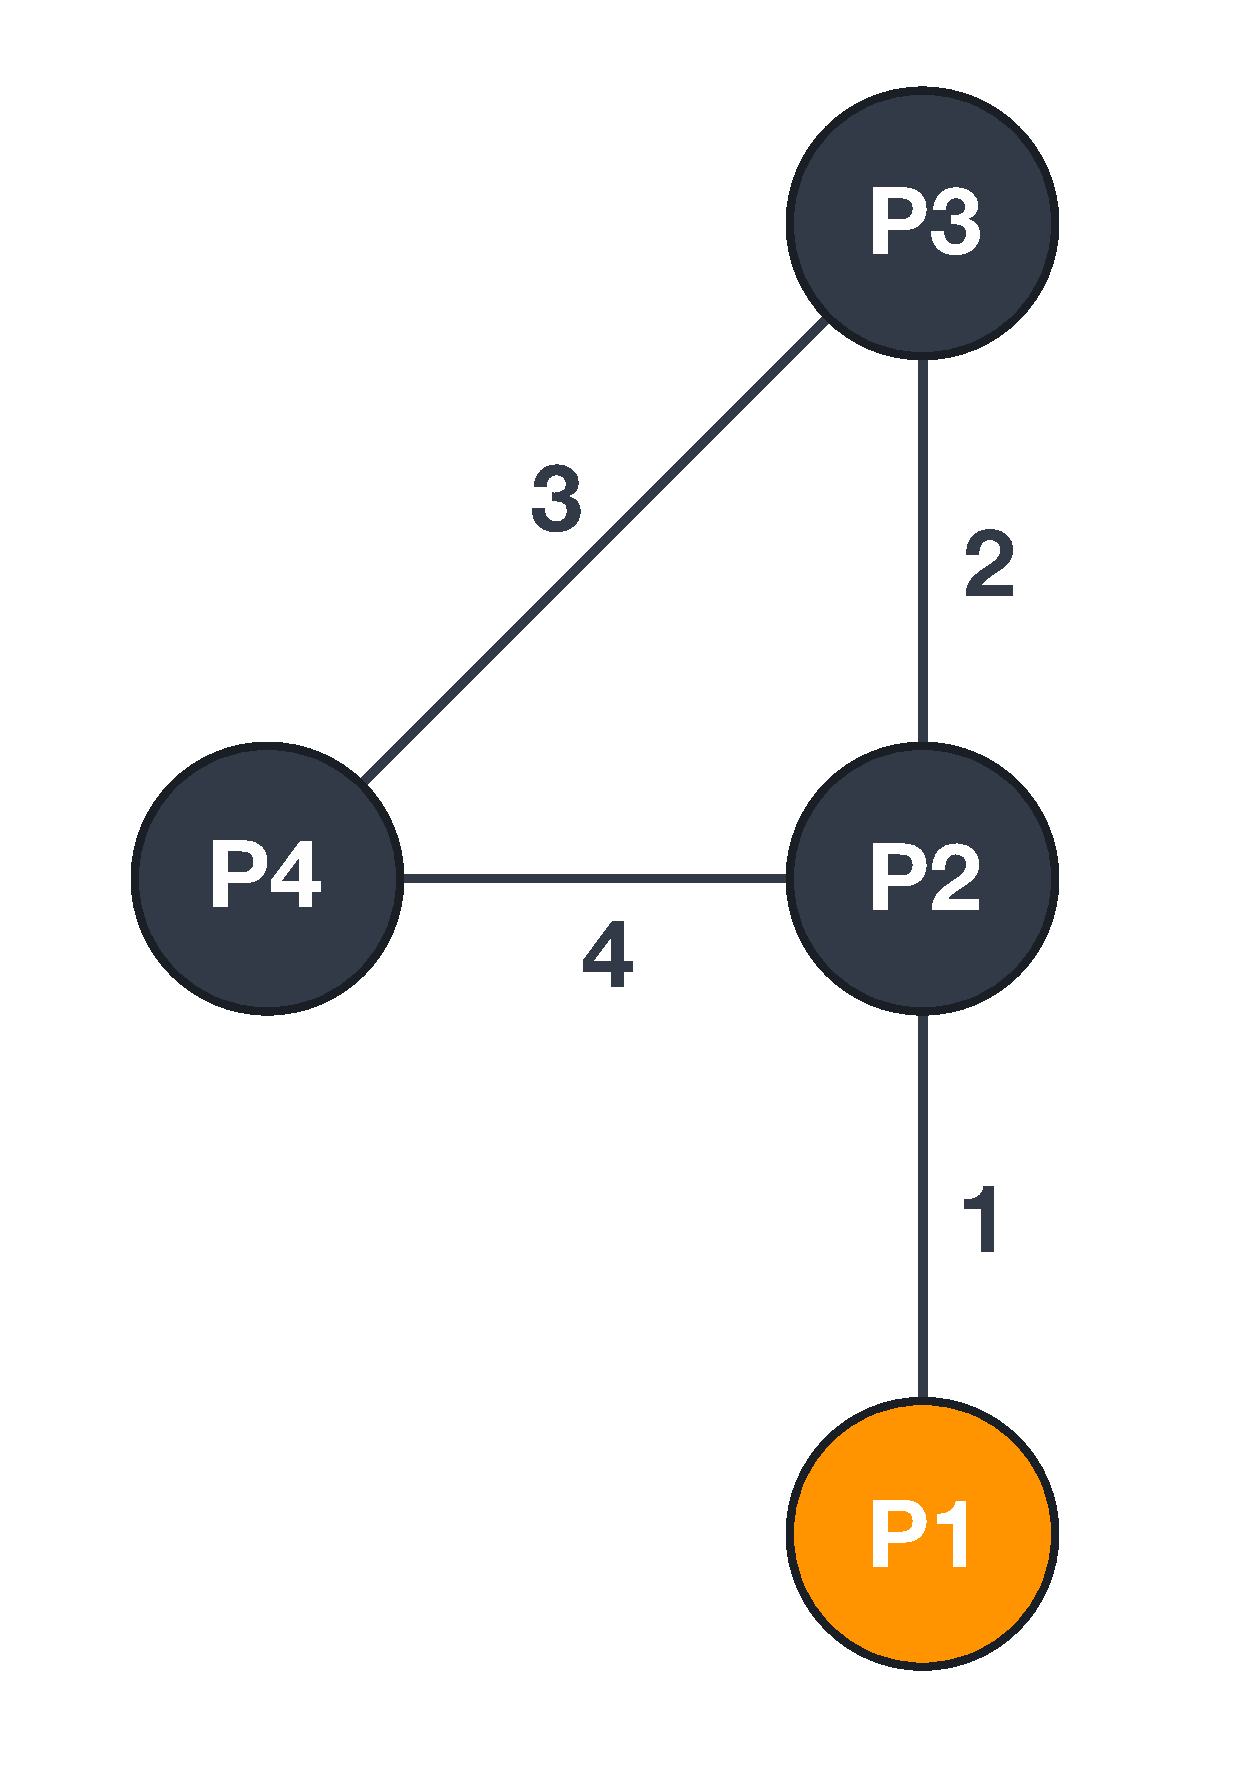
\includegraphics[width=0.5\textwidth]{schema.pdf}
\caption{Schemat systemu wraz z oznaczeniem procesorów}
\label{fig:schema}
\end{figure}

Biorąc pod uwagę fakt, że węzeł $P1$ jako jedyny  posiada dane w stanie początkowym może on odgrywać jedynie rolę nadawcy danych.
Węzeł $P2$ może zarówno otrzymywać (z węzła $P1$), jak i nadawać dane (do węzłów $P3$ i $P4$). Na łączu 1 komunikacja będzie się odbywać w kierunku “do” węzła P2,
natomiast na łączach 2 i 4 będzie się odbywać w kierunku “z” węzła $P2$. Niestety, nie możemy w modelu ogólnym założyć, czy dana komunikacja wystąpi.
Trzeba pamiętać, że komunikacja na łączach 2 i 4 ma szanse wystąpić tylko jeśli wystąpi komunikacja na łączu 1 (węzeł $P2$ otrzyma dane z węzła $P1$).
Komunikacja na łączu 1 (pomiędzy węzłami $P1$ i $P2$) nie musi wystąpić jeśli koszt transmisji danych na tym łączy będzie stosunkowo duży.
W przypadku węzłów $P3$ i $P4$ warto zauważyć symetrię \ref{fig:symetry}. Przyjęliśmy, że komunikacja odbywać będzie się na łączu 3 zawsze w kierunku
od $P3$ do $P4$. Aby zrealizować odwrotną komunikację należy zamienić procesory $P3$ i $P4$ oraz łącza 2 i 4.


\begin{figure}[!ht]
\centering
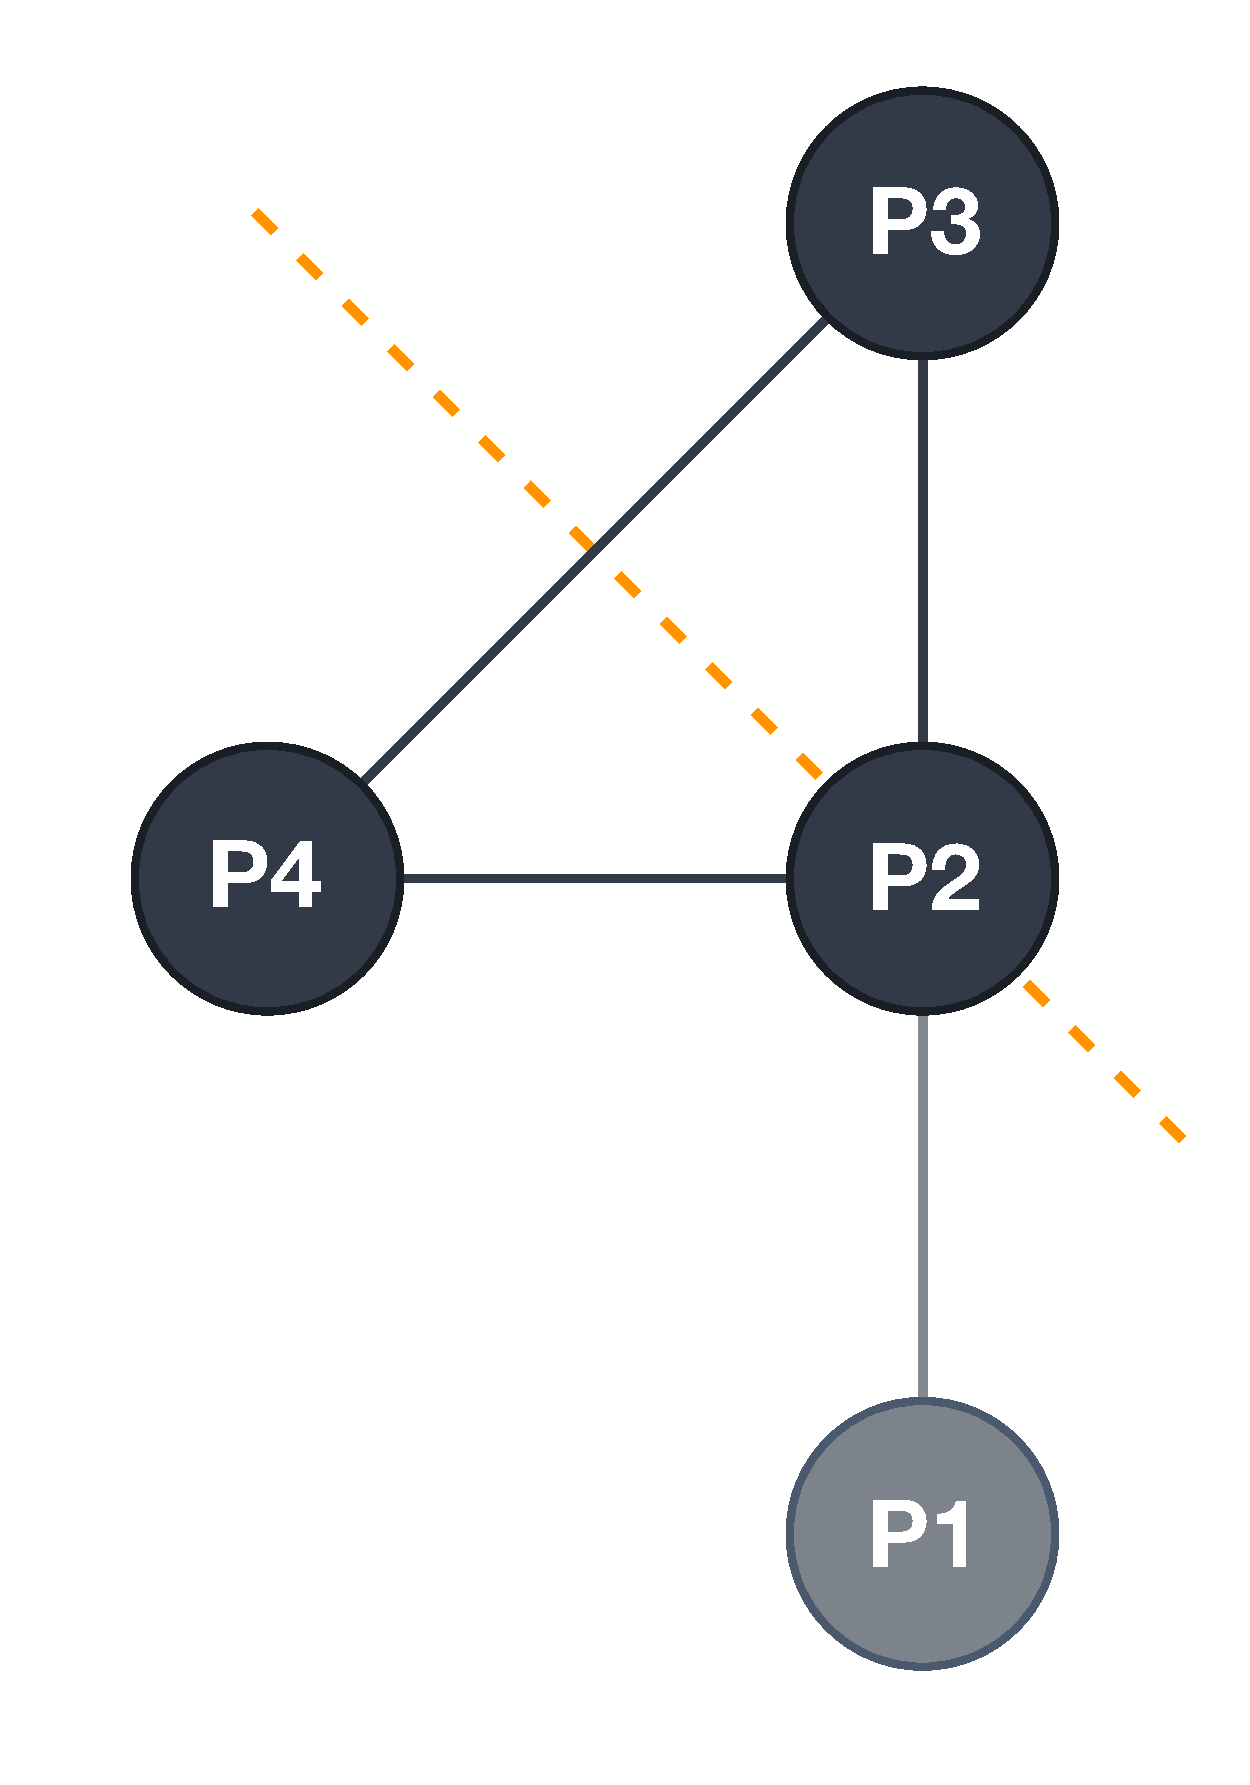
\includegraphics[width=0.5\textwidth]{symetry.pdf}
\caption{Symetria w analizowanym systemie (oznaczona linią przerywaną)}
\label{fig:symetry}
\end{figure}

W przypadku modeli sekwencyjnych transmisja pomiędzy urządzeniami może się odbyć tylko i wyłącznie gdy oba nie wykonują żadnych obliczeń i nie uczestniczą w innej komunikacji.
W przypadku zrównoleglenia obliczeń dopuszczalna jest jednoczesna komunikacja danego procesora z więcej niż jednym urządzeniem
oraz dokonywania obliczeń na danych znajdujących się na tymże procesorze.
Zważając na fakt, że porcje danych są liczbami całkowitymi należy mieć na uwadze konieczność synchronizacji urządzeń. \\

Dla każdego z modeli minimalizowana jest wartość $T$, która jest większa bądź równa od wszystkich wartości $T_{x}$ (czas zakończenia wszystkich działań na procesorze $Px$) gdzie $x = 1, 2, 3, 4$.
 
\subsection{Analiza modelu sekwencyjnego}

Przetwarzanie w systemie bez zrównoleglenia podzieliliśmy na 3 modele, w zależności od kolejności przesyłania danych na poszczególnych łączach.
W każdym z modeli jako pierwsza występuje komunikacja na łączu $P1 \to P2$. Następnie odbywają się komunikacje na łączach $P2 \to P3$, $P2 \to P4$ oraz $P3 \to P4$.
Komunikacje te mogą występować w różnej kolejności z uwzględnieniem, że komunikacja $P2 \to P3$ musi wystąpić przed komunikacją $P3 \to P4$ (jeśli w ogóle występuje).
W analizowanym systemie w danej chwili komunikacja może odbywać się jedynie na jednym łączu, ponieważ w każdej z komunikacji bierze udział węzeł $P2$.

\subsubsection{Pierwszy model sekwencyjny}

Model ten zakłada kolejność komunikacji: $P1 \to P2$, $P2 \to P4$, $P2 \to P3$ oraz $P3 \to P4$. \\

\begin{description}

\item[Węzeł $P1$] \hfill \\

Działanie procesora $P1$ polega na wysłaniu do $P2$ danych przetwarzanych przez inne procesory a następnie przetworzeniu pozostałych danych.
Jeśli prędkość komunikacji na tym łączu będzie odpowiednio mała lub pozostałe procesory będą wolne to komunikacja na tym łączu nie wystąpi
i $P1$ przetworzy wszystkie dane w systemie. Jeśli z kolei łącze 1 będzie szybkie lub procesory $P2$, $P3$, $P4$ będą szybkie
lub procesor $P1$ będzie wolny to czas pracy procesora $P1$ może sprowadzić się do wysłania danych do procesora $P2$.

\item[Węzeł $P2$] \hfill \\

Jeśli wystąpi komunikacja między $P1$ i $P2$ to w ogólnym przypadku czas zakończenia pracy procesora $P2$ można ustalić jako sumę czasu komunikacji na łączu $P1 \to P2$,
czasu komunikacji na łączu $P2 \to P4$, czasu komunikacji na łączu $P2 \to P3$ oraz obliczeń na tym procesorze.
Jeśli któraś z tych komunikacji nie wystąpi to czas pracy tego procesora będzie odpowiednio krótszy.

\item[Węzeł $P3$] \hfill \\

Jeżeli wystąpi komunikacja między $P2$ i $P3$ to czas zakończenia pracy $P3$ można ustalić jako sumę czasu komunikacji na łączu $P1 \to P2$,
czasu komunikacji na łączu $P2 \to P3$, obliczeń pomiędzy komunikacjami, czasu bezczynności (koniecznego do synchronizacji z $P4$), komunikacji $P3 \to P4$ oraz obliczeń po komunikacji.
Obliczenia między komunikacjami wynikają z faktu, że jednocześnie z komunikacją $P2 \to P3$ mogą odbywać się obliczenia na procesorze $P4$
które muszą zakończyć się po obliczeniu całkowitej porcji danych i jednocześnie przed rozpoczęciem komunikacji $P3 \to P4$.
Opłacalne może okazać się obliczenie części danych na procesorze $P3$ przed rozpoczęciem nadawania danych do $P4$. \\

Podczas analizy systemu łatwo zauważyć, że gdy szybkości procesorów i łącz są zrównoważone to przypadek z pominięciem komunikacji $P3 \to P4$ występuje najczęściej,
gdyż między $P2$ i $P4$ jest bezpośrednie połączenie.
Ciekawy jest przypadek w którym węzeł $P3$ nie przeprowadza żadnych obliczeń, a jedynie pośredniczy w komunikacji między $P2$ i $P4$.
Występuje on m.in. gdy łącza $P2 \to P3$ i $P3 \to P4$ są dostatecznie szybkie, a procesor $P3$ jest wolny.

\item[Węzeł $P4$] \hfill \\

Czas zakończenia pracy procesora $P4$ jest w dużej mierze zależny od pracy procesora $P3$. Po zakończeniu odbioru danych od $P2$ procesor może rozpocząć obliczenia,
ponieważ konieczna jest synchroniazacja z $P3$ (możliwe, że kosztem bezczynności).
Jeśli komunikacja $P3 \to P4$ występuje, to pierwsza część obliczeń kończy się przed jej rozpoczęciem. Po zakończeniu tej komunikacji rozpoczyna się druga część obliczeń. \\

Warto zauważyć, że gdyby obliczenia mogły być przerwane w dowolnym momencie (a nie tylko po obliczeniu całkowitej ilości danych),
to obliczenia między odbiorem danych od $P2$ i odbiorem danych od $P3$ zawszy by występowały (jeśli odpowiednie komunikacje miały by miejsce).

\end{description}

\subsubsection{Drugi model sekwencyjny}

Model ten zakłada kolejność komunikacji: $P1 \to P2$, $P2 \to P3$, $P3 \to P4$ oraz $P2 \to P4$. \\

\begin{description}

\item[Węzeł $P1$] \hfill \\

Działanie procesora $P1$ jest analogiczne do działania procesora $P1$ w modelu 1.

\item[Węzeł $P2$] \hfill \\

Procesor $P2$ po otrzymaniu danych od $P1$ rozpoczyna wysyłanie danych do $P3$, a następnie w czasie komunikacji $P3 \to P4$ oblicza pierwszą część danych.
W czasie tych obliczeń ma miejsce komunikacja $P3 \to P4$. Z powodu konieczności obliczenia całkowitej porcji danych obliczenia mogą trwać dłużej niż komunikacja
między $P3$ i $P4$. W szczególności na procesorze $P4$ po zakończeniu tej komunikacji mogą rozpocząć się obliczenia.
Konieczna jest zatem synchronizacja między procesorami (możliwe, że kosztem chwilowej bezczynności), po której następuje komunikacja $P2 \to P4$ i pozostałe obliczenia.

\item[Węzeł $P3$] \hfill \\

\item[Węzeł $P4$] \hfill \\

\end{description}

\subsubsection{Trzeci model sekwencyjny}

\begin{description}

\item[Węzeł $P1$] \hfill \\

Działanie procesora $P1$ jest analogiczne do działania procesora $P1$ w modelu 1.

\item[Węzeł $P2$] \hfill \\

\item[Węzeł $P3$] \hfill \\

\item[Węzeł $P4$] \hfill \\

\end{description}

\subsection{Analiza modelu równoległego}

Analiza modelu równoległego.


\subsubsection{Pierwszy model równoległy}

\begin{description}

\item[Węzeł $P1$] \hfill \\

\item[Węzeł $P2$] \hfill \\

\item[Węzeł $P3$] \hfill \\

\item[Węzeł $P4$] \hfill \\

\end{description}

\subsubsection{Drugi model równoległy}

\begin{description}

\item[Węzeł $P1$] \hfill \\

\item[Węzeł $P2$] \hfill \\

\item[Węzeł $P3$] \hfill \\

\item[Węzeł $P4$] \hfill \\

\end{description}
